\section{Malacology: A Programmable Storage System}

\begin{figure}[tb]
\centering
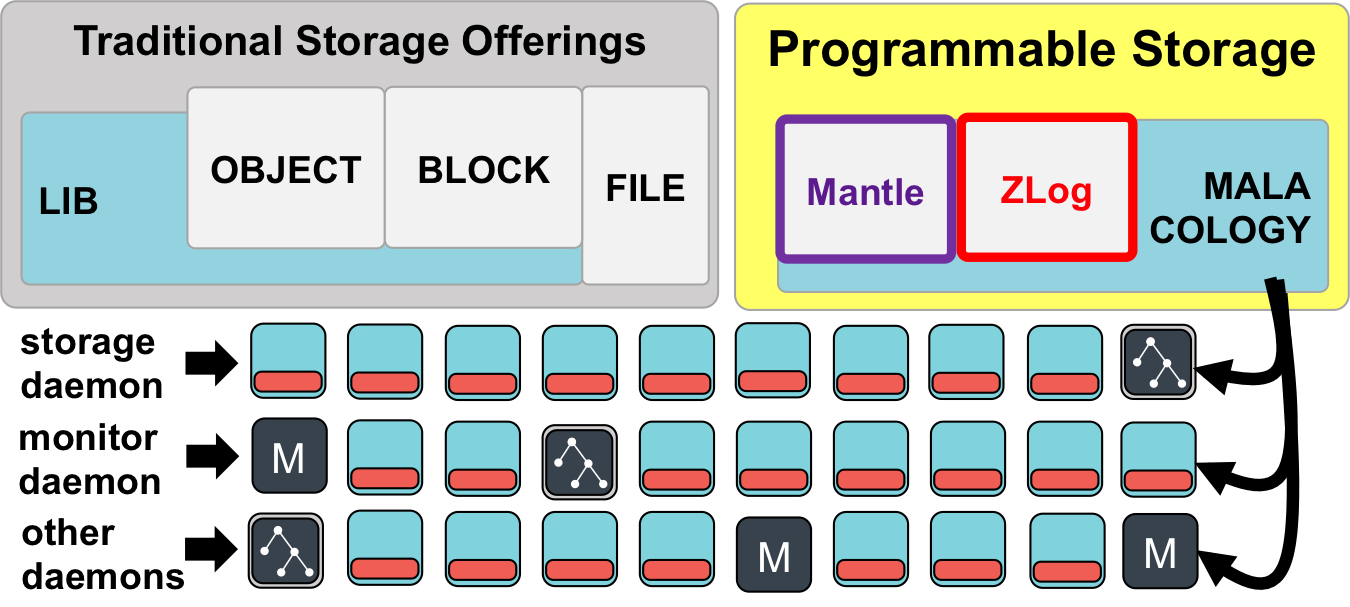
\includegraphics[width=0.7\textwidth]{./chapters/background/figures/overview.png}
\caption{Scalable storage systems have storage daemons which store data,
monitor daemons (M) that maintain cluster state, and service-specific daemons
({\it e.g.}, MDSs). Malacology enables the programmability of
internal abstractions (bold arrows) to re-use and compose existing subsystems.
With Malacology, we built new higher-level services, ZLog and Mantle, that sit
alongside traditional user-facing APIs (file, block,
object).}\label{fig:overview}
\end{figure}

Malacology is a programmable storage system built on Ceph. A programmable
storage system facilitates the re-use and extension of existing storage
abstractions provided by the underlying software stack, to enable the creation
of new services via composition. Programmable storage differs from
\emph{active storage}~\cite{riedel:vldb98}---the injection and execution of
code within a storage system or storage device---in that the former is
applicable to any component of the storage system, while the latter focuses on
the data access level. Given this contrast, we can say that active storage is
an example of how one internal component (the storage layer) is exposed in a
programmable storage system.

Malacology was built on Ceph because Ceph offers a broad spectrum of existing
services, including distributed locking and caching services provided by file
system metadata servers, durability and object interfaces provided by the
back-end object store, and propagation of consistent cluster state provided by
the monitoring service (see Figure~\ref{fig:overview}).  Malacology includes a
set of interfaces that can be used as building blocks for constructing novel
storage abstractions, including:

\begin{enumerate}

\item An interface for managing strongly-consistent time-varying
\textbf{service metadata}.

\item An interface for installing and evolving domain-specific, cluster-wide
\textbf{data I/O} functionality.

\item An interface for managing access to \textbf{shared resources} using a
variety of optimization strategies.

\item An interface for \textbf{load balancing} resources across the cluster.

\item An interface for \textbf{durability} that persists policies using the
underlying storage stack's object store.

\end{enumerate}

These interfaces are core to other efforts in programmable storage, such as
DeclStor~\cite{watkins:hot17-declstor, watkins:techreport16-brados}, and were
built on a systematic study of large middleware
layers~\cite{watkins_invivo_2013, watkins:scc2012-datamods}.  Composing these
abstractions in this way potentially jeopardizes the correctness of the system
because components are used for something other than what they were designed
for. To address this, we could use something like lineage-driven fault
injection~\cite{alvaro:sigmod15-ldfi} to code-harden a programmable storage
system like Malacology.
